%
% main.tex
%
% This file contains only the skeleton of the technical note:
%  * package import and setup
%  * page setting
%  * author list
%  * title page
% 
% The rest of the content is imported from other files.
%


\documentclass{article}

% \usepackage[margin=1in]{geometry} 
\usepackage{amsmath,amsthm,amssymb,amsfonts}
\usepackage{float}
\usepackage{graphicx}
\usepackage{fancyhdr}
% \usepackage{url}           % for on-line citations
% \usepackage{bm}            % special 'bold-math' package 
% \usepackage{graphics}      % standard graphics specifications
\usepackage{authblk}  % allows more complex multi-author, multi-affiliation author list
\usepackage{natbib}   % bibliography as Overleaf likes
\usepackage{upgreek}  % \upmu...

% \usepackage[dvipsnames,table]{xcolor}
% \usepackage{subfig}


%for the links
% \usepackage{color}
\usepackage{hyperref}
\hypersetup{
    colorlinks=true, % make the links colored
    linkcolor=blue, % color TOC links in blue
    urlcolor=red, % color URLs in red
    linktoc=all
    } % 'all' will create links for everything in the TOC

\usepackage{cleveref} % \cref and \Cref for "clever" reference text; needs to be loaded after hyperref

% \usepackage{sectsty}
% \subsectionfont{\fontsize{12}{15}\selectfont\centering}
% \sectionfont{\fontsize{12}{15}\selectfont\centering}
% \renewcommand\thesection{\Roman{section}}
% \renewcommand\thesubsection{\Alph{subsection}}
% \renewcommand{\familydefault}{\updefault}

% Set up fancy header/footer
\pagestyle{fancy}
\fancyhead[LO,L]{T600 Detector}
\fancyhead[CO,C]{\title{}}
\fancyhead[RO,R]{}
\fancyfoot[LO,L]{}
\fancyfoot[CO,C]{\thepage}
\fancyfoot[RO,R]{}
% \renewcommand{\headrulewidth}{0.4pt}
% \renewcommand{\footrulewidth}{0.4pt}

\providecommand{\tightlist}{%
  \setlength{\itemsep}{0pt}\setlength{\parskip}{0pt}}

%%%%%%%%%%%%%%%%%%%%%%%%%%%%%%%%%%%%%%%%%%%%%%%%%%%%%%%%%%%%%%%%%%%%%%%%%%%%%%%%
%%% Macro definitions
%%%

% physics quantities
\newcommand{\micros}[1]{\ensuremath{#1}\,\ensuremath{\upmu{}}s}
\newcommand{\Hz}[1]{\ensuremath{#1}\,Hz}
\newcommand{\V}[1]{\ensuremath{#1}\,V}
\newcommand{\milliV}[1]{\ensuremath{#1}\,mV}
\newcommand{\mebiB}[1]{\ensuremath{#1}\,MiB}


%%%%%%%%%%%%%%%%%%%%%%%%%%%%%%%%%%%%%%%%%%%%%%%%%%%%%%%%%%%%%%%%%%%%%%%%%%%%%%%%
%%% Front page definition
%%%


\title{ICARUS connectivity test}


\author[a]{Brenda~G\'omez \thanks{gomez.cortes14@gmail.com}}
\affil[a]{Universidad de Colima}

\author[b]{Angela~Fava \thanks{afava@fnal.gov}}
\affil[b]{Fermi National Accelerator Laboratory}

\author[c]{Mark~Convery \thanks{convery@slac.stanford.edu}}
\author[c]{Gianluca~Petrillo \thanks{petrillo@slac.stanford.edu}}
\author[c]{Yun-Tse~Tsai \thanks{yuntse@slac.stanford.edu}}
\affil[c]{SLAC National Accelerator Laboratory}

\author[z]{Somebody~else \thanks{somebody@institution.edu}}
\author[z]{adding the others is a to-do \thanks{of course}}
\affil[z]{Someone's institution}

\date{\today}


%%%%%%%%%%%%%%%%%%%%%%%%%%%%%%%%%%%%%%%%%%%%%%%%%%%%%%%%%%%%%%%%%%%%%%%%%%%%%%%%
\begin{document}

\maketitle

\label{abstract}

\begin{abstract}
  We present here the procedure and results of the connectivity tests done on the TPCs wire planes of the ICARUS detector.
  All three, In\-duc\-tion-1, In\-duc\-tion-2 and Collection planes were tested.
  A test pulse was injected to each wire and an output signal was obtained and measured.
  An off-site analysis of the output signal waveforms was carried out for all standard and non-standard chimneys.
  As a result of the tests, we present a detailed description and mapping of how the detector is done from inside.
\end{abstract}



\tableofcontents

\section{Introduction}
\label{sec:Introduction}


Here goes an introduction to the document with a description of the structure and the content of each section. This may be the last part to be written, i.e. after all sections are completed.



\section{T600 Detector -- TPC (Time Projection Chamber)}
\label{sec:Detector}

detector done from inside.....


%To tests all the $53258$ wires that make up the whole ICARUS TPC without actually going inside the detectors it was decided to pull the connectors outside from the cryostat flanges through all the chimneys, to carefully and methodically inject a test pulse to the pulser cables that are directly connected to a board at the bottom of the vessel. To the same board is connected a single flat ribbon of 32-twisted cables connector that corresponds to only 32 wires of the TPC (Fig.). On top of the wire plane there's another board connected to another flat ribbon of those same 32 wires. This is the connector that then goes plugged-in to a test box. 



\section{Wire Connectivity Tests}
\label{sec:TheTest}

The main goal of the ICARUS TPC's connectivity tests here described has been to check the condition of the wires of the each anode plane of the detector; i.e., to look/check for wires not properly working or even disconnected. \\

The tests, as described in \cref{ssec:stand_chimn}, were done using a test box that sends a pulse of specific voltage, triggers the oscilloscope and receives back an output signal from the wires and sends it to oscilloscope where we can look and measure the expected peak and amplitude.\\

Since horizontal cables can't get a pulse injected, there was a slightly different procedure to test the 8 non-standard chimneys (See \cref{ssec:nonStd_chimn}). 


\subsection{Test box}
\label{ssec:TestBox}

The SLAC test box (Fig.) was designated specially for the ICARUS TPC wire plane connectivity tests. It's a portable battery powered device with dimensions $20\times 15\times 10$ cm.\\

\begin{figure}[htb]
\centering
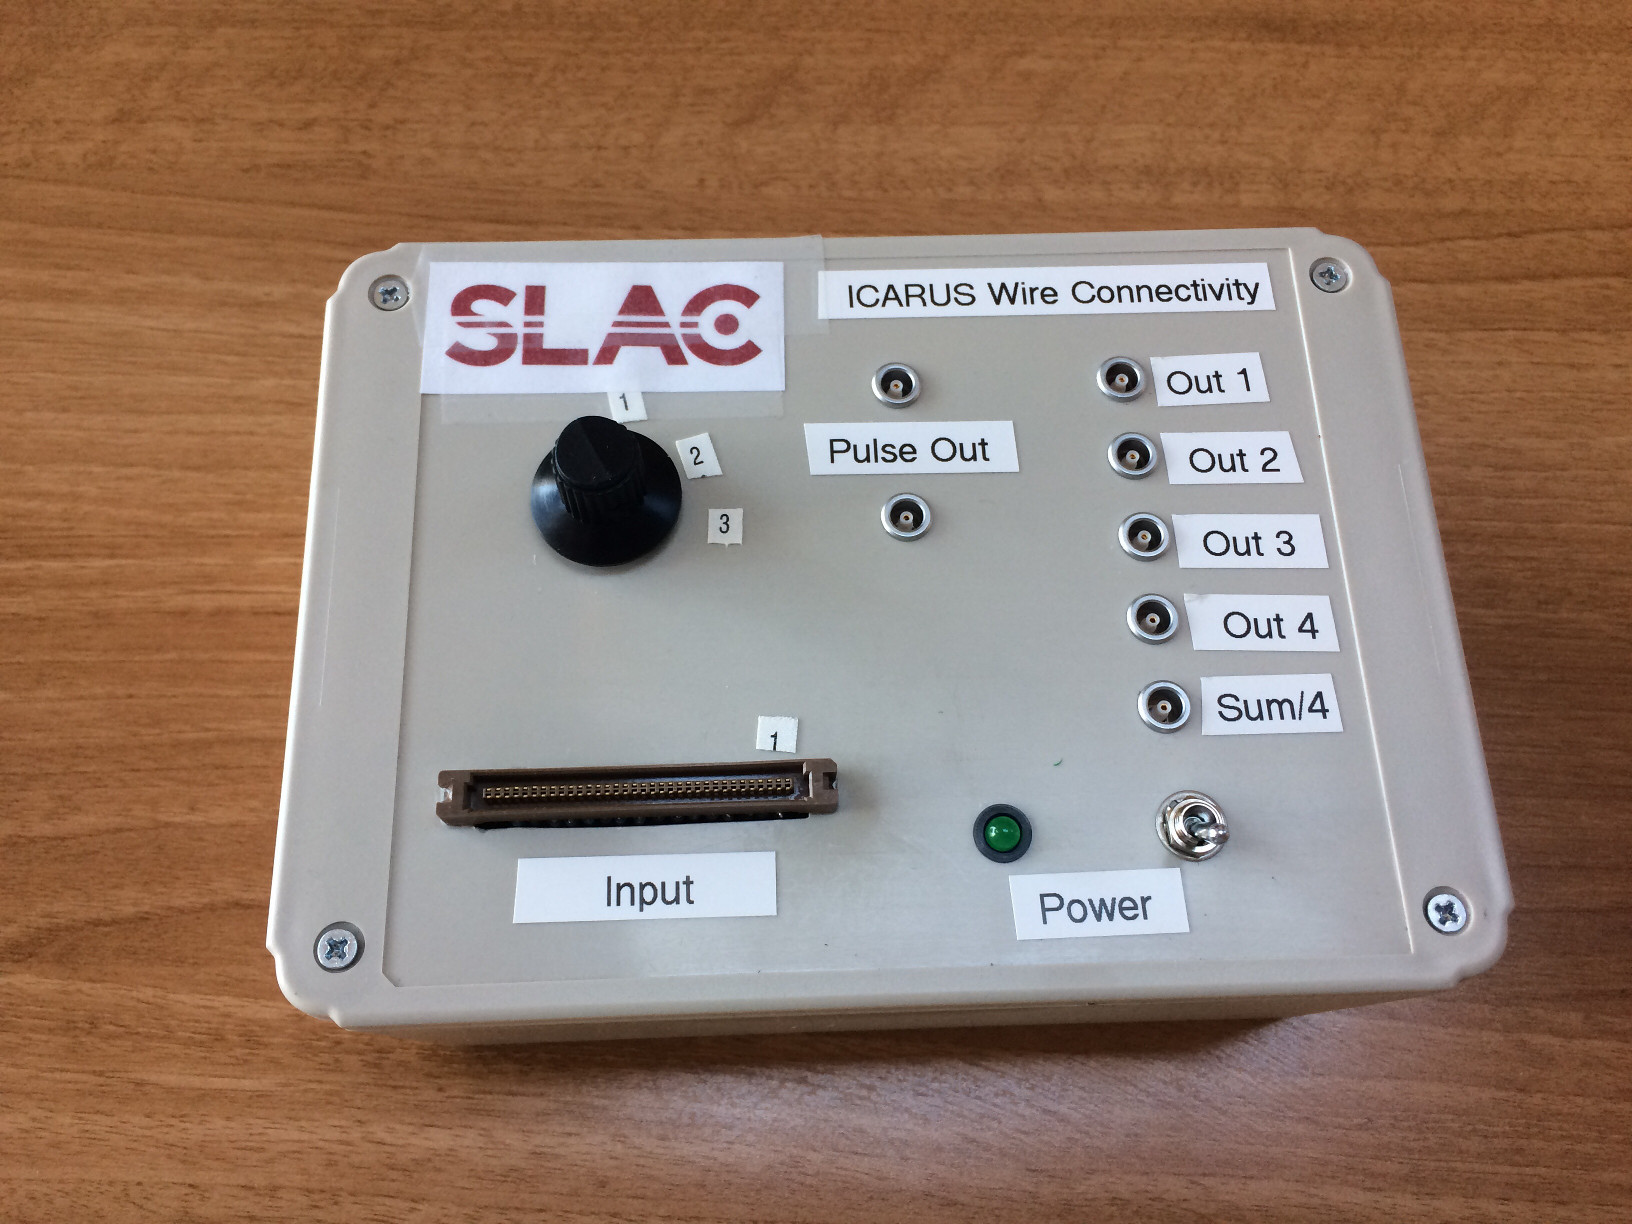
\includegraphics[width=0.8\linewidth]{fig/box1}
\caption{SLAC test box version 1}
\end{figure}

On the lid it contains:
\begin{itemize}
\item Built in pulser outputs on LEMO with both polarities,
\item Connector for a single flat ribbon of twisted-pairs cable: TPC cables plug into this connector with all grounds connected together.
\item An 8-position rotary switch that switches all 4 channels at a time,
\item The test pulse: $100$ Hz, $5$ V, $1 \mu $s rise time, $100 \mu $s length.

Two test boxes were built. It was found out that the cable shields, although connected together, were not grounded in the box. This was observed as a full size signal of about $1.5$ V.  The second version of the box contains extra outputs that allowed us to ground the shields of the connectors (Fig. second box). 
\end{itemize}

%SPEND MORE WORDS (regarding schematics of the electronics inside) ON THE TEST BOX!!!!



\subsection{Standard Chimneys}
\label{ssec:stand_chimn}

%The standard chimneys of the detector are the 2 to 19 $1$m tall cylinders that are bolted to the flanges on top of the cryostats (Fig.).

%\begin{figure}[H]
%\centering
%\includegraphics[scale=0.1]{fig/chimn}
%\caption{Chimneys installed, view from south to north.}
%\end{figure}

The TPC cables were pulled out from the detector through all the chimneys (Fig.) and the tests were performed in the following way: \\


%THIS PARAGRAH/INFO goes in Part II.
%The standard chimneys contain $18$ flat ribbon connectors each, $8$ pulser cables, groups of cables that belongs to the photomultipliers (High Voltage and signal) and optical fibers.\\

%\begin{figure}[H]
%\centering
%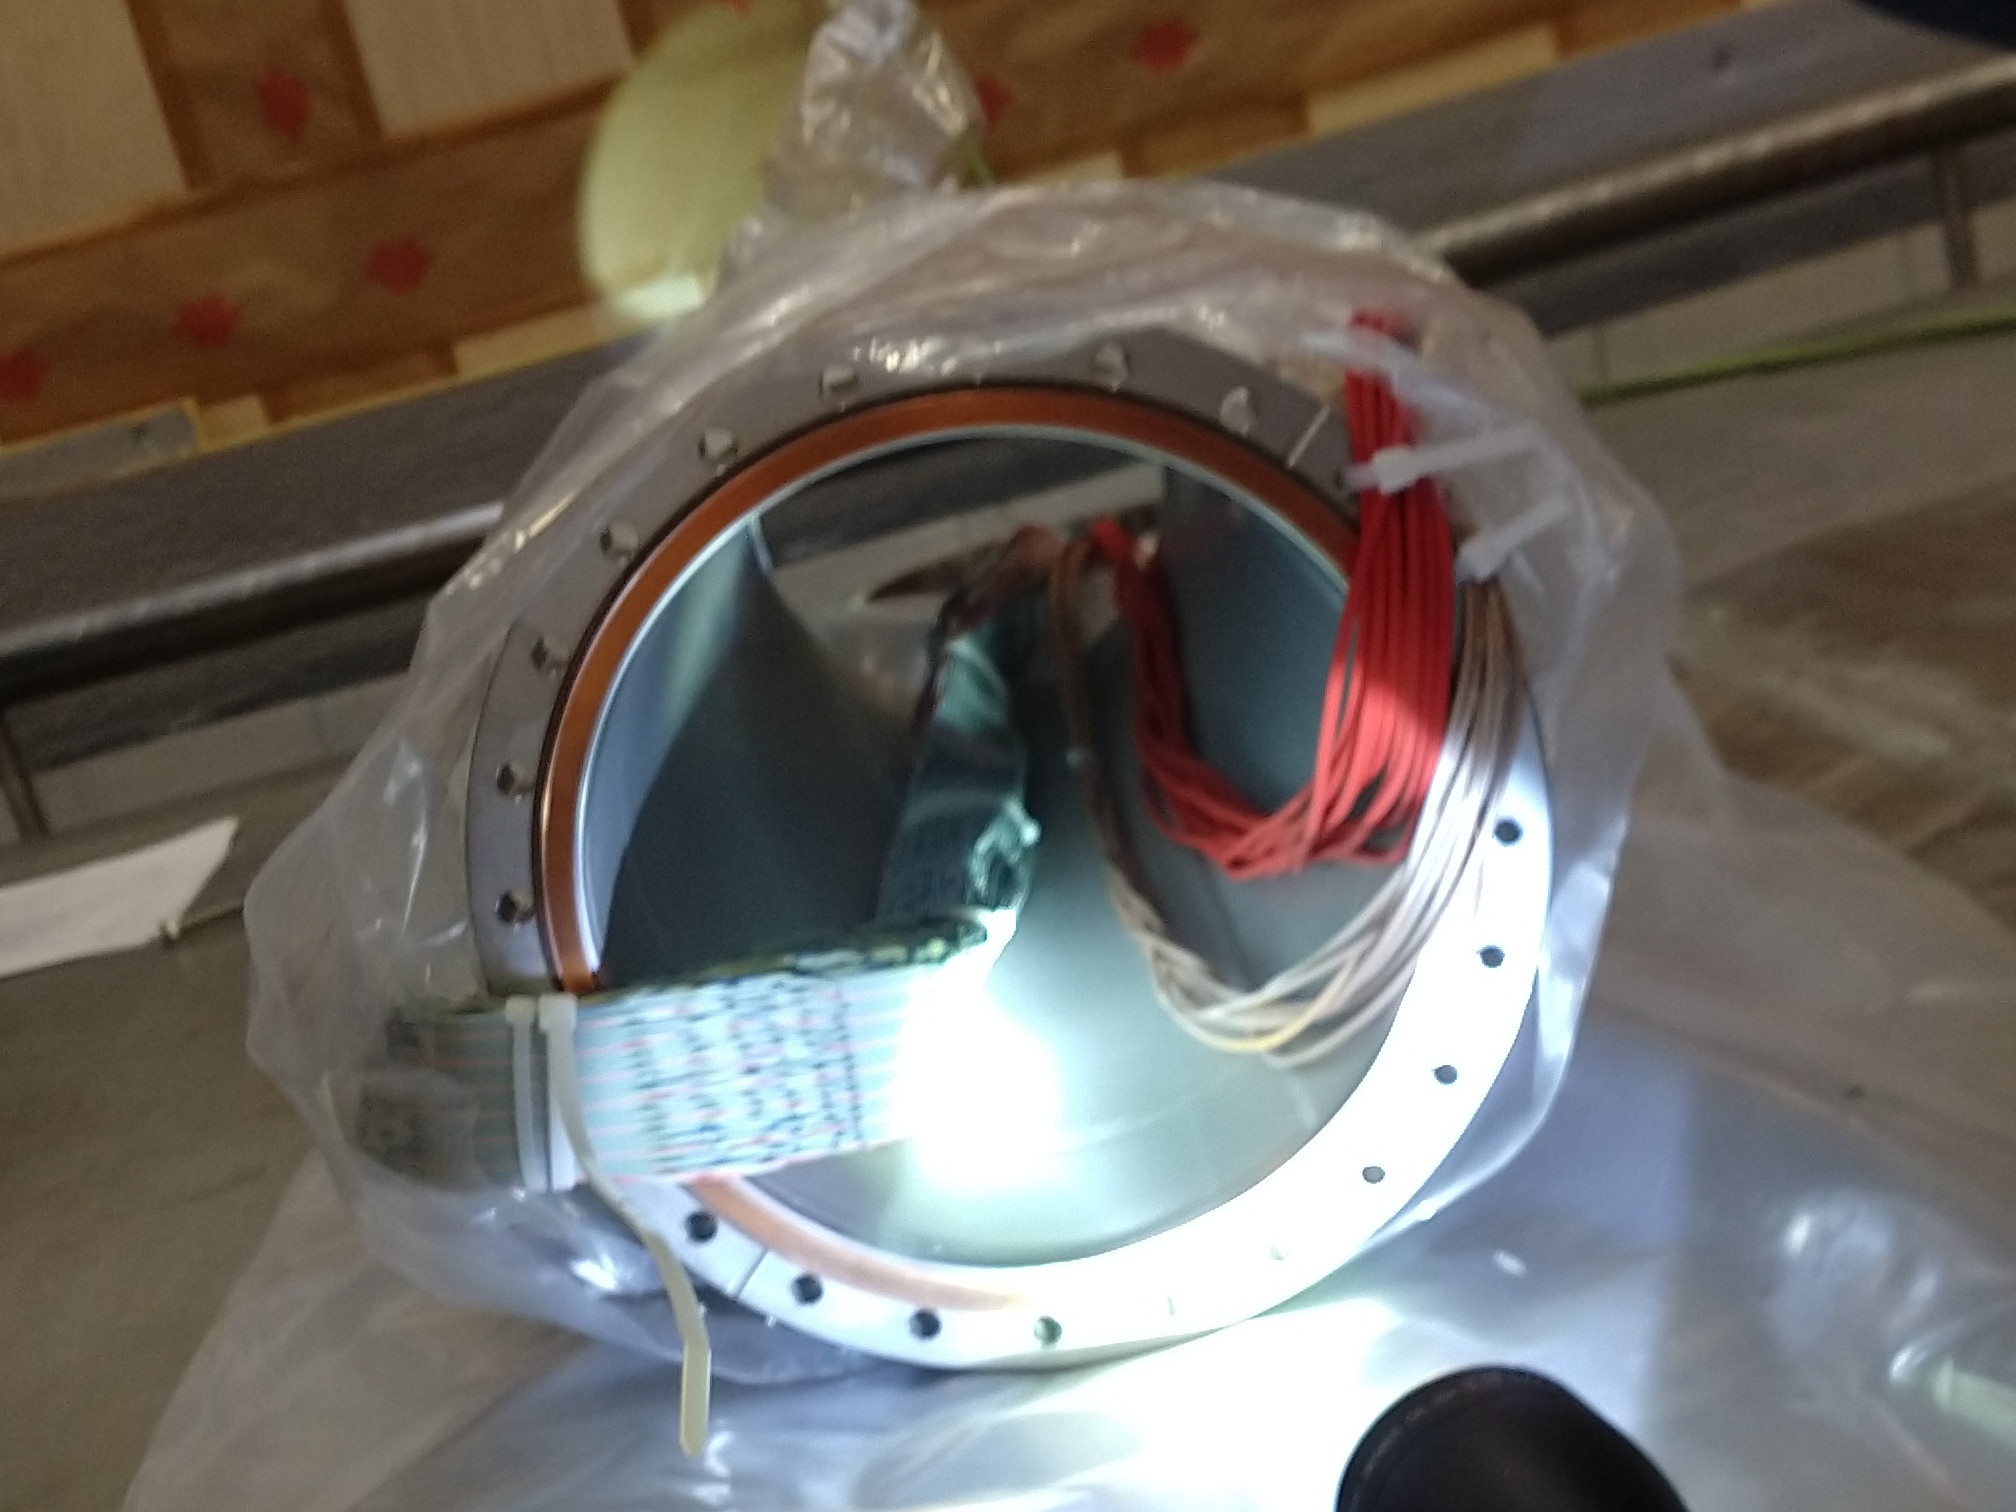
\includegraphics[scale=0.06]{fig/cab1} 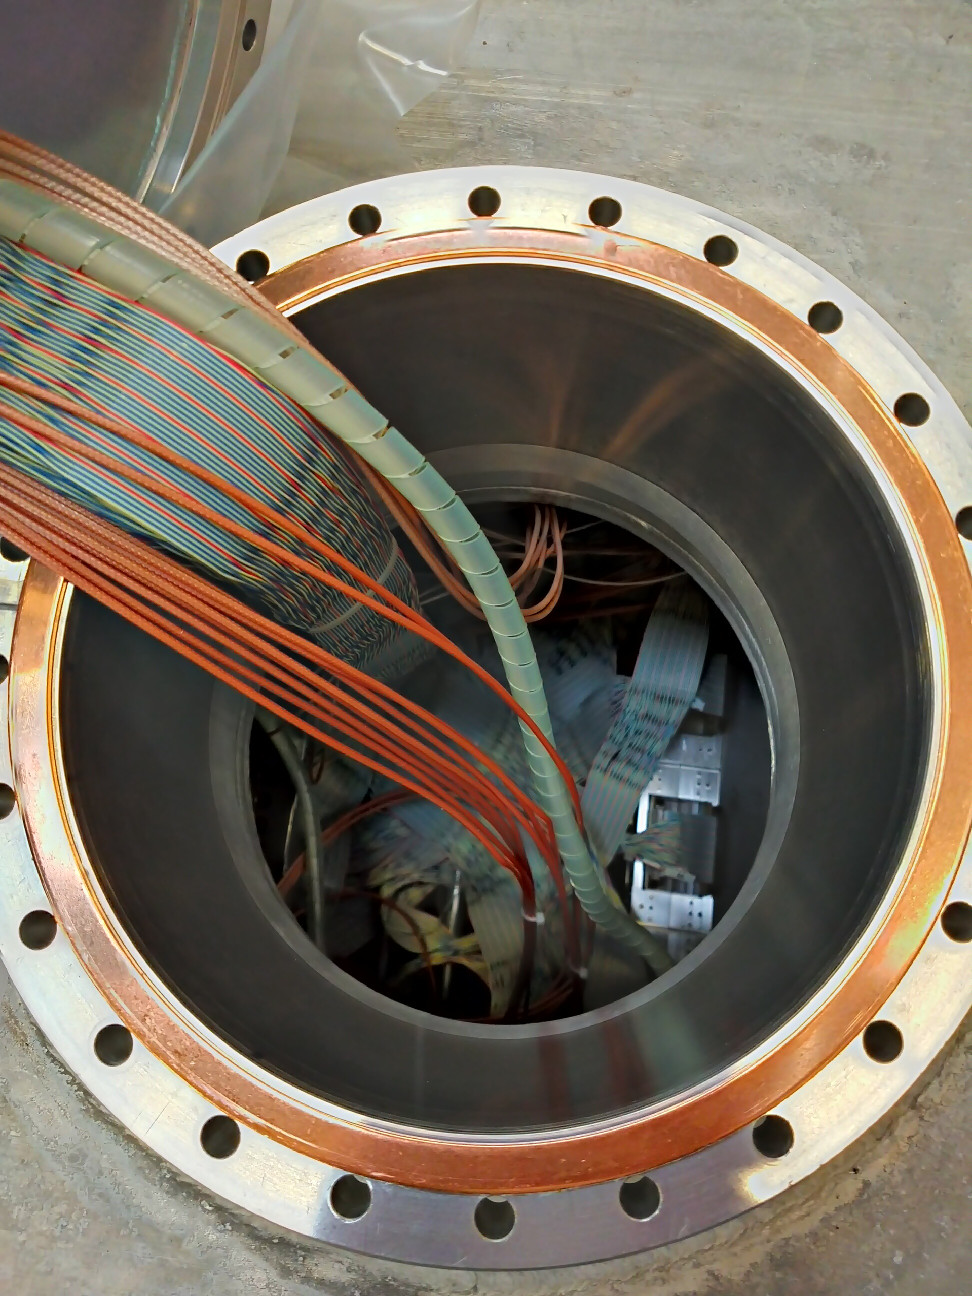
\includegraphics[scale=0.08]{fig/cab2}
%\caption{Left: Installation of a chimney. Right: HV PMT's cables (red), TPC connectors (colored flat ribbon cables)}
%\end{figure}


%Also this lines go in Part II
%The cables of interest are:
 
%\begin{itemize}
%\item 4 of the 8 SMA cables, the ones with red tag,

%\begin{figure}[H]
%\centering
%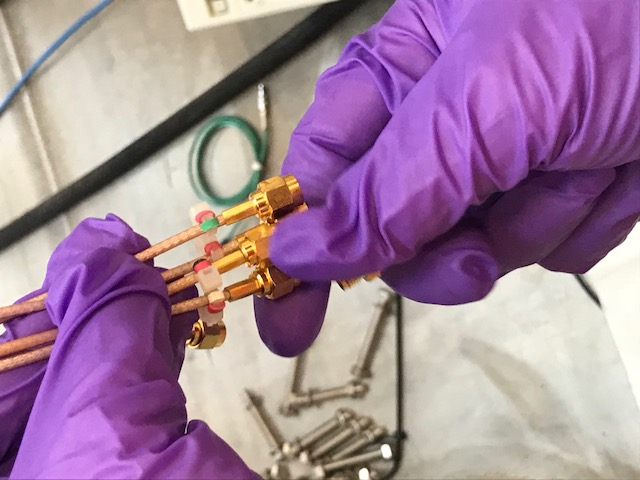
\includegraphics[scale=0.3]{fig/SMA} 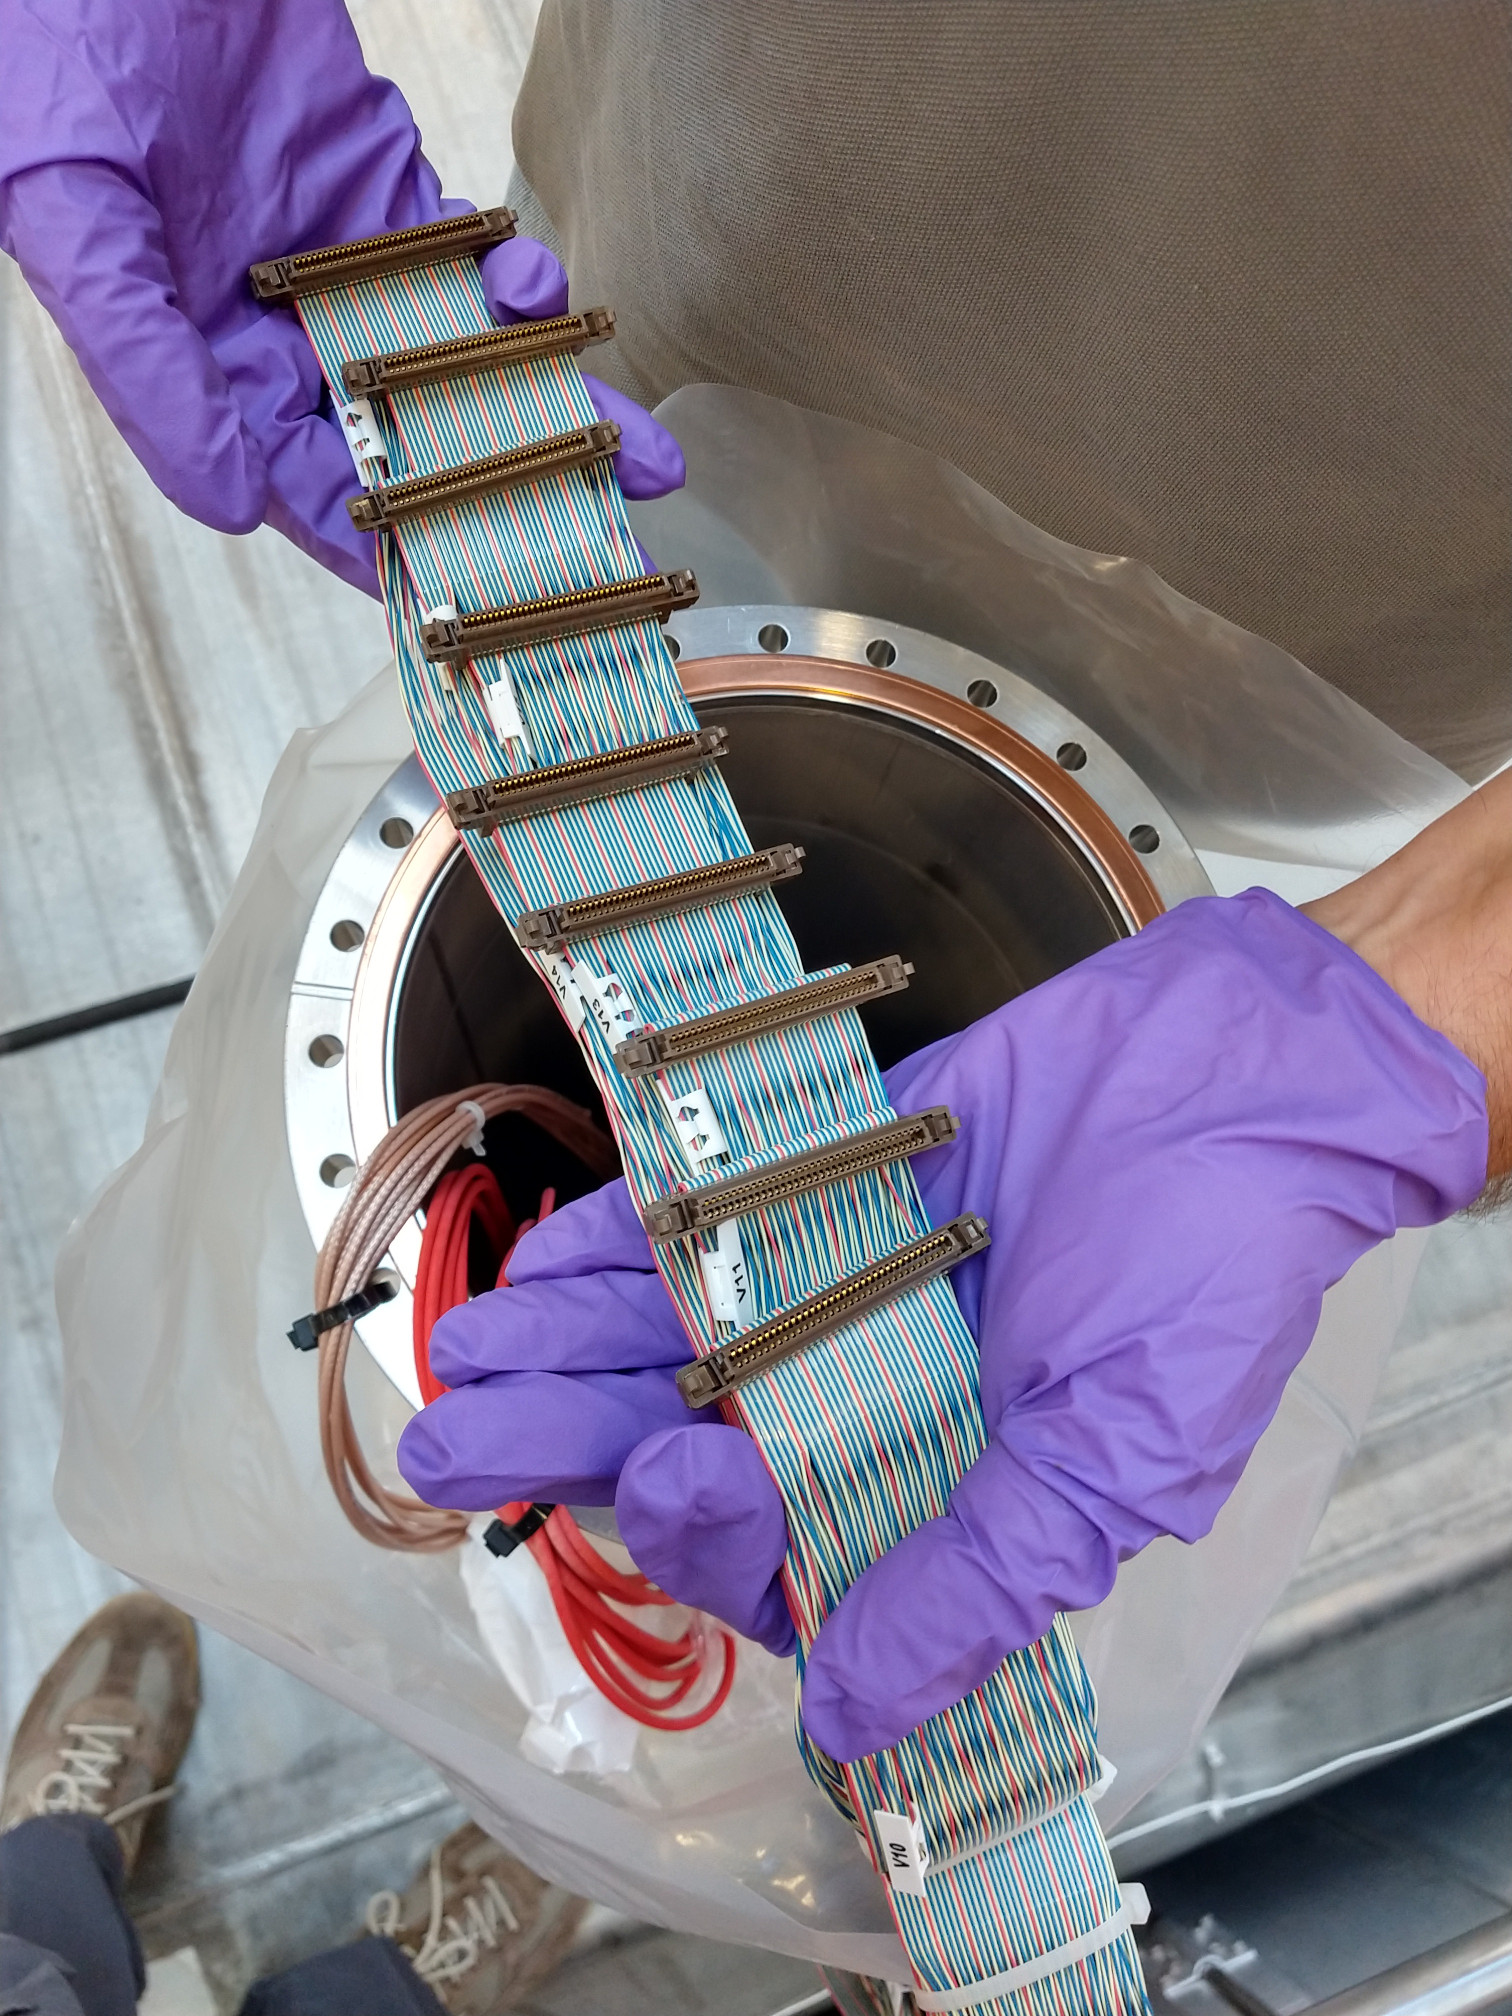
\includegraphics[scale=0.05]{fig/conn1}
%\caption{Left: SMA pulser cables, Right: 32 TPC wires per each single flat ribbon of twisted-pairs cables.}
%\end{figure}

%\item the $18$ flat ribbon connectors.

%\end{itemize}

\textit{Procedure:}\\
\begin{enumerate}
\item The external trigger was connected from one of the test-pulse output of the box to the oscilloscope (at the back). Therefore, the setting for the trigger in the oscilloscope input was changed to: "EXT" (external).

\item 4 LEMO cables connected from the box to the four inputs of the oscillope correspond to four channels of the signal (Fig.).

\item A SMA-female coaxial cable goes connected on the "pulse-out" of the box via LEMO conection and the SMA-female side is connected to the pulser from the detector.

An important requirement before starting to take data was to test all 4 SMA cables (red tag) in the search for the highest pulse.

In order to verify that everything was working properly, the box was tested in-site by connecting the test-pulse output directly to one channel of the oscilloscope, with the settings changed to DC and $1$ M$\Omega $ and looked for the $5$ V square signal on the screen. In addition, we verified the SMA (from the detector) to LEMO (pulser cable from the box) connection by using a chain of LEMO to SMA-female plus SMA-male to LEMO to connect the test box to the oscilloscope.

\item For a systematic test, we chose to start from the cable S/V18 to S/V1. Since the test box injects and receives output signal from only 4 cables of a single flat ribbon connector, we had to swith through 8 positions with the black know on top of the box in order to test all 32 wires from 1 connector at a time. 

\item The waveforms seen on the screen of the oscilloscope were downloaded using a Python script written by S. Castells [ref] and stored in an external disk for an offsite analysis. 


\begin{figure}[H]
\centering
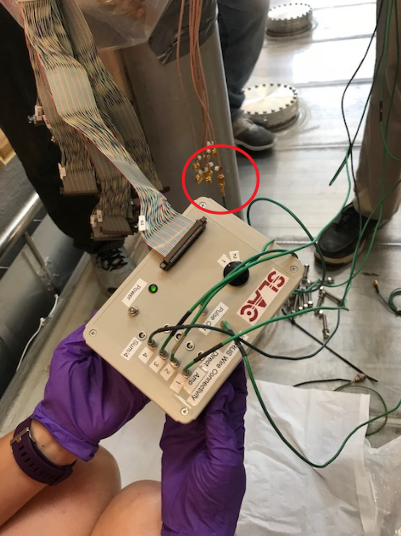
\includegraphics[scale=0.6]{fig/setup}
\caption{Set up of the hardware components. The red circle shows the SMA to LEMO connectors through which the box injects the test pulse.}
\end{figure}




\end{enumerate}




\subsection{Non-standard chimneys}
\label{ssec:nonStd_chimn}

The non-standard chimneys are the 8 corners of both cryostats, see Fig. Apart from the difference in size between standard and non-standard chimneys, the latter ones contain the horizontal and corner wire connectors. \\

As described on \cref{sec:Detector} the configuration of the horizontal wires does not allow to inject a pulse directly to the wires and therefore a different way to test them was developed. \\
The test pulse was injected to 32 wires of Induction-2 plane at once. From one standard chimney, two or three chimneys away from the corner, a connector between 2 and 9 was choosen and plugged in to a board (<-name?). To pulse those 32 wires we use the same conexion from the test box: a chain LEMO to SMA cables and to one of the 4 red-tagged pulser cables from the chimney.  


\subsection{Waveforms retrieval}
\label{ssec:DAQ}

I will add the procedure for the retrieval and the code used?



\section{Waveform analysis}
\label{sec:Analysis}


A fast data analysis was performed within hours or days from the data
acquisition. Each waveform is analysed individually, through a few
steps:

\begin{itemize}
\tightlist
\item
  baseline identification: average of the central 50\% of the samples
\item
  RMS: RMS of the samples used in the baseline determination
\item
  extrema determination: amplitude of the positive and negative peaks
  along the whole waveform
\end{itemize}


For each channel, the parameters from all the available waveforms (10)
are averaged to extract:

\begin{itemize}
\tightlist
\item
  baseline RMS (RMS of the 10 baselines)
\item
  noise average (average of the 10 RMS, one for of each baseline)
\item
  peak amplitude average and its uncertainty (the positive
  peak from each waveform are averaged)
\end{itemize}

This analysis is aimed for speed, and it can definitely be refined.

% ----------------------------------------------------------------------
\subsection{Baseline and RMS identification}
\label{sec:baseline-and-rms-identification}


The principle is to exclude the signal, intended as the response to the
pulse, and to use the remaining of the waveform to estimate the
baseline. The algorithm is designed not to require prior knowledge of
the position or shape of the peaks.\\

The signal is shaped as two sharp-rising peaks, which including the
decay tails are roughly 200 µs or shorter. The algorithm relies on the
assumption that those two peaks are indeed roughly that narrow, although
it does not assume anything on their size or shape. It flows as follows:

\begin{enumerate}
\tightlist
\item
  sort all the 10000 samples in increasing order; in this way, the
  samples taken during the negative peak will be at the left of the
  data, the ones at the positive peak will be at its right, and the
  middle of the data will be populated by long sequences of samples with
  similar values, from the baseline
\item
  select the samples from \#2500 to \#7499 from the sorted data for
  further analysis
\item
  take the average and RMS of the selected samples, which will represent
  the baseline and noise respectively
\end{enumerate}

This algorithm may present some bias if the tail from the first peak
overlaps the second peak. An alternative, simple algorithm would rely on
the assumption that the peak is on the second half of the waveform, and
would therefore use the first 40\% or 50\% of the waveform for baseline
determination as in the last point of the algorithm.\\

An older version of the algorithm would rely of the knowledge of the
peak position, and would fail when the waveform does not contain any
actual signal.


% ----------------------------------------------------------------------
\subsection{Peak determination}
\label{sec:peak-determination}


Again a simple algorithm, the peak determination consists of two simple
steps:

\begin{enumerate}
\tightlist
\item
  determine the absolute maximum and minimum of the waveform
\item
  subtract to both the baseline (obtained separately)
\end{enumerate}

This algorithm is affected by the noise on the waveform, which can be
quantified together with the baseline. Although this is less than ideal,
the actual noise has been measured to be low enough to be not
significant for the purpose of the fast analysis we performed{[}1{]}.\\

{[}1{]} In more recent versions of the library, the minimum and maximum
are not evaluated from the single sample, but replaced by a running
window average on 5 samples.


% ----------------------------------------------------------------------
\subsection{Results}
\label{sec:results}

We summarize the results of the baseline, RMS, positive peak value, 
and the ratio of the positive peak value to the baseline in 
\Cref{fig:baseline,fig:rms,fig:pospeak,fig:pospeaktobaseline}.
Each strip represents a single channel of the detector.
The x-axis includes all the chimneys of the ICARUS detector, while
the y-axis shows all the 18 cables, each with 32 channels, within a chimney.
The color code in each figure indicates the values of the baseline, the RMS,
the positive peak, or the ratio of the positive peak value to
the baseline value.\\

The corner chimneys, Ch01 and Ch20 in each row, have only the channels
connecting to horizontal wires, where the data was not recorded in this
round of the connectivity test and therefore is not shown in the plots.
Cables 1-9 in Ch02 and Ch03 and cables 10-18 in Ch18 and Ch19 are connected
to the corner wires in the second induction and collection planes which are
shorter in length.
Owing to their ending points, the cables injecting the test pulse are
not located at the same chimney.
Without the information of the location of the pulse-injecting cables,
we are not able to obtain a result of these wires, and 
\Cref{fig:pospeak,fig:pospeaktobaseline} show extremely low or
overflown values.\\


% ----------------------------------------------------------------------
\begin{figure}
\centering
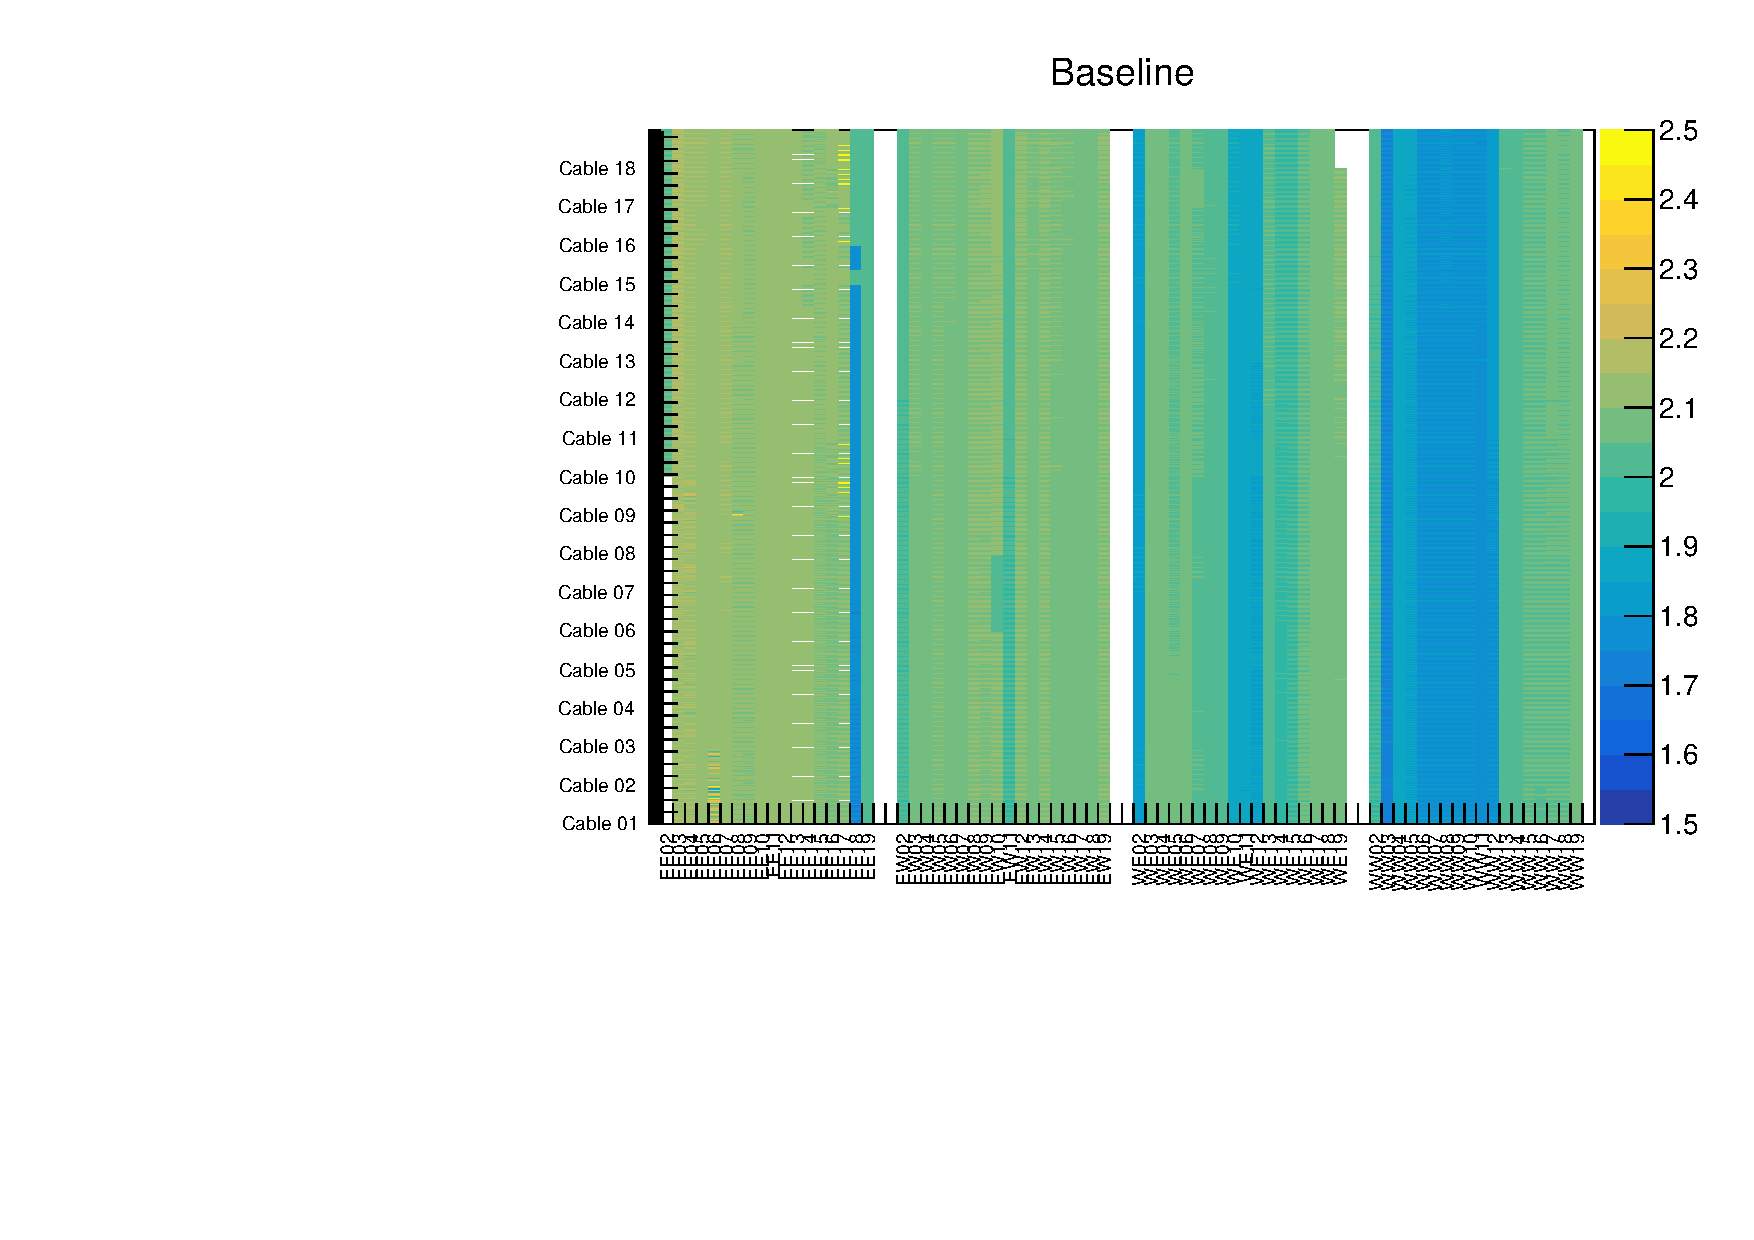
\includegraphics[width=\textwidth]{fig/Baseline.pdf}
\caption{The map of the baseline values of all the channels.
Each strip represents a single channel of the detector.
The x-axis includes all the chimneys of the ICARUS detector, while
the y-axis shows all the 18 cables, each with 32 channels, within a chimney.
The color code in each figure indicates the values of the baseline.}
\label{fig:baseline}
\end{figure}
% ----------------------------------------------------------------------

% ----------------------------------------------------------------------
\begin{figure}
\centering
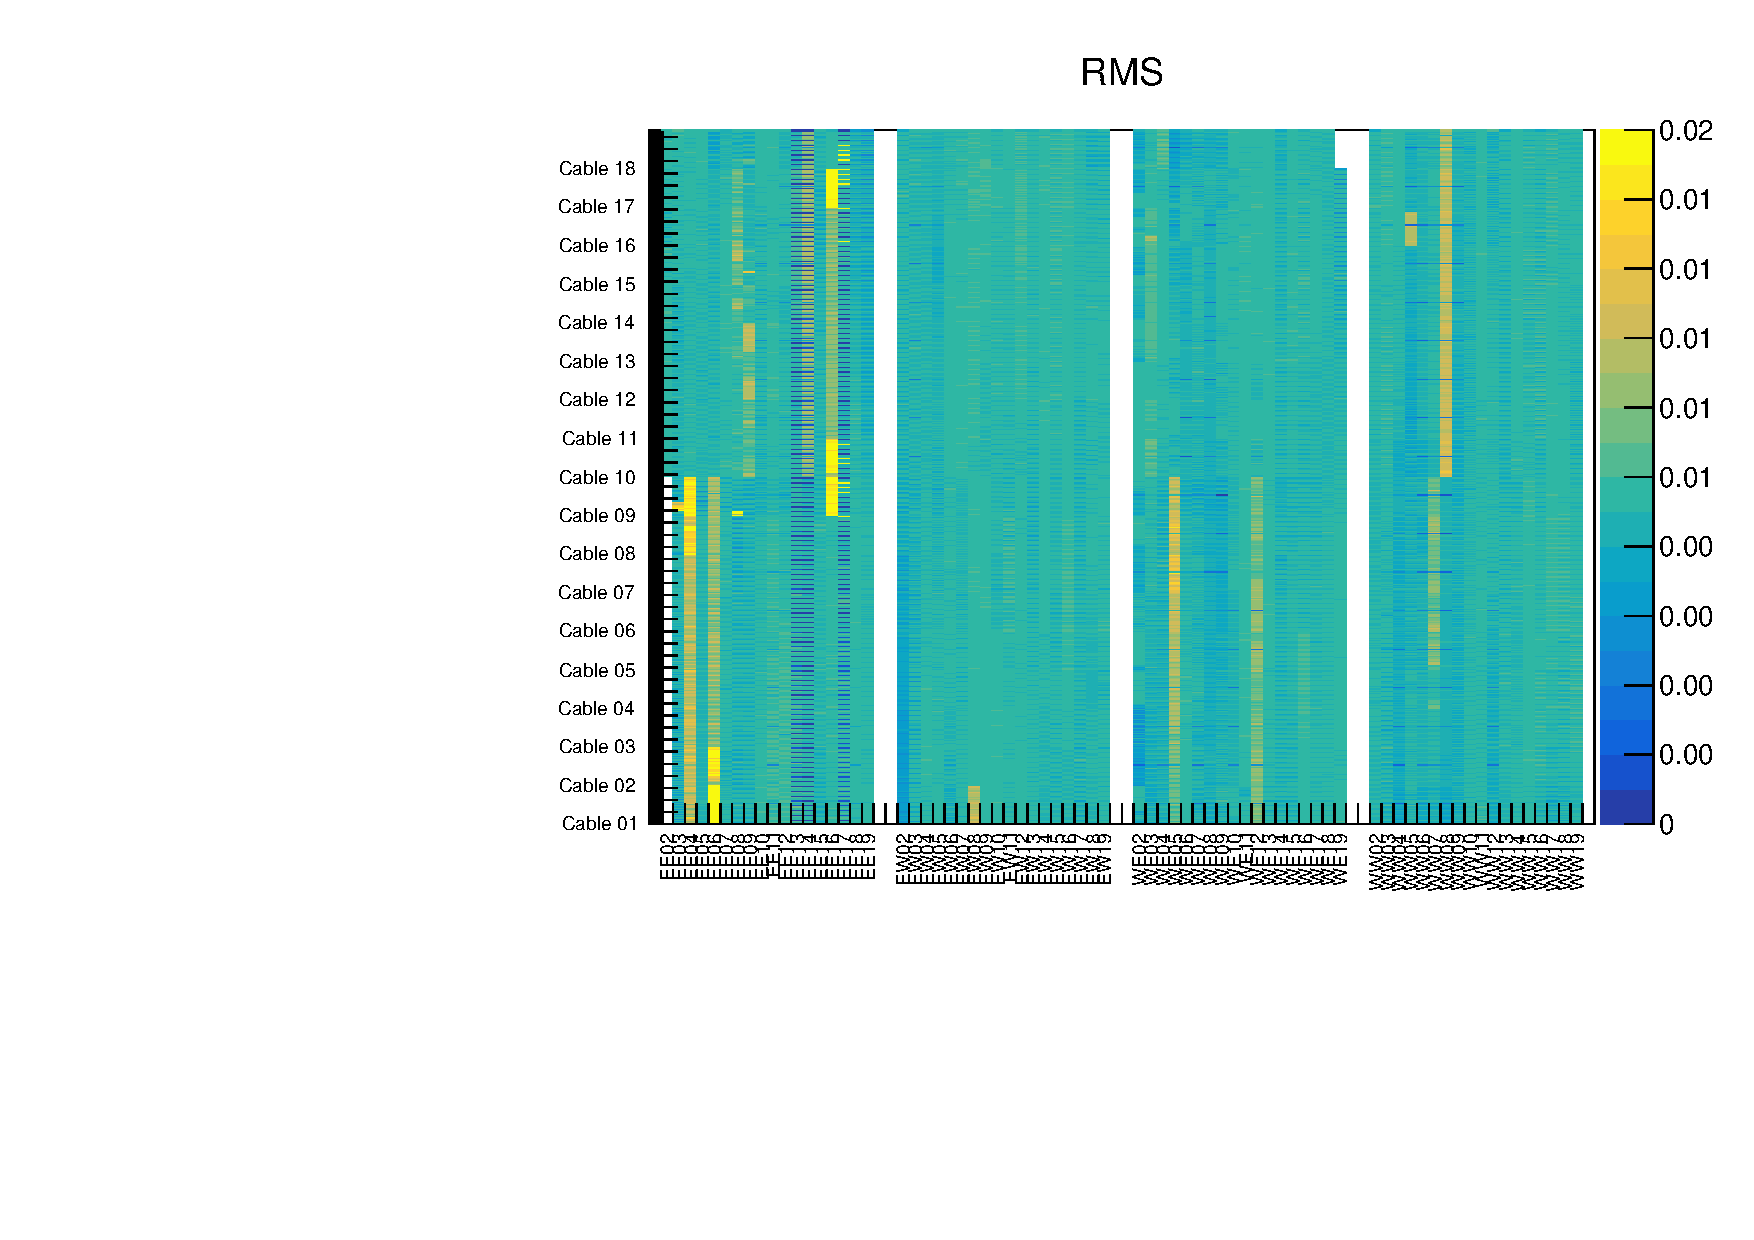
\includegraphics[width=\textwidth]{fig/RMS.pdf}
\caption{The map of the RMS of all the channels.
Each strip represents a single channel of the detector.
The x-axis includes all the chimneys of the ICARUS detector, while
the y-axis shows all the 18 cables, each with 32 channels, within a chimney.
The color code in each figure indicates the values of the RMS.}
\label{fig:rms}
\end{figure}
% ----------------------------------------------------------------------

% scale in the oscilloscope
In chimneys EE13, EE14, and EE17, the white strips in \Cref{fig:baseline} 
and the dark blue strips in \Cref{fig:rms,fig:pospeak},
indicating extremely low values,
appear in every four channels.
It is owing to the fact that the fourth channel in the oscilloscope
happens to be set a larger scale in voltage, and, as a consequence, 
the relative values of the baseline and the pulse peak are small.
The effect is canceled out in \Cref{fig:pospeaktobaseline}, where the
ratio of the peak to baseline values is plotted.\\

% dead channel in the test box
The fifth channel of the connector for the flat ribbon cables in a test
box is damaged, and we are not able to read out the signals from the
channel when using this test box.
It thereby shows the dark blue strips in chimneys EE10-14, EW 03-07,
WE02-12, and WW03-12 in \Cref{fig:pospeak,fig:pospeaktobaseline}.
Nonetheless, this round of the connectivity test aims to identify
potential problems in terms of cables, and a single damaged channel
in the test box should not affect the effectivity.\\

% voltage
Since there is no voltage regulator for the battery powering the test
boxes, the baseline value, which is set to the half of the voltage,
decreases as the time being, as shown in \Cref{fig:baseline}.
Hence, \Cref{fig:pospeaktobaseline}, which cancels out the baseline
decrease, gives us a more uniform comparison across the whole detector.\\

% special cables
In the EE and WE rows, cables 1-8, cable 9, cables 10-17, and cable 18
have separate pulse-injecting cables, while in the EW and WW rows, those
groups are cable 1, cables 2-10, cable 11, and cables 12-18.
During the tests, we do not have the information on this grouping of
wires, except that cables 1-9 and 10-18 are for induction and collection
wires, respectively, and have different pulse-injecting cables.
Consequently, for some chimneys, cables 1-9 are tested with
the same pulse-injecting cable, and so are cables 10-18; 
for other chimneys, cables 1-8, 10, 11-17, and 18 are tested with different
pulse-injecting cables.
With the cross talk effect discussed in the next paragraph,
it is not straightforward to distinguish whether the measured signal
corresponds to the injected pulse or the cross talk signal in the special
cables, cables 9 and 18 in the EE and WE chimneys and cables 1 and 11
in the EW and WW chimneys.
In addition, it is raised that the grouping of the channels for the same
pulse-injection cables might be cables 1-8, 9, 10-17, 18 for the chimney
EE02, but cables 1, 2-10, 10-17, 18 for the next chimney, EE03, and
similar patterns for other chimneys.
However, we have not reached a conclusive statement by analyzing the
current data, which convolved several issues including the cross talk,
potentially wrong cables for pulse-injection, etc.
We defer the conclusion to the next iteration of connectivity test
where we expect to have equipment disentangling those issues.\\

% cross talk
The wires involved in the connectivity test should normally not be connected
to the detector ground, but it was observed that some of them are during the
overhaul at CERN.
The design of the test box in this iteration does not connect the wire cables
to the detector ground, and therefore in the normal case of the wire grounding,
the cross talk from the adjacent twisted wires contributes a significant
portion to the signal.
Roughly speaking, the amplitude of the cross talk signal is similar to
to that of the injected pulse, which severely complicates the signal
interpretation.
In the normal case, where the wire is correctly connected but not grounded 
to the detector, the signal will be the superposition of the injected
pulse and the cross talk signal.
On the other hand, in the cases that the wire is not connected and not
grounded, and that the wire is connected and also grounded,
the signal will contain, respectively, only the cross talk and only the
injected pulse, both of which will have roughly half the amplitude of
the signal in the normal condition.
By analyzing all the possible scenarios listed in \Cref{table:crosstalk},
we ensure the connectivity of the channels with the full size amplitude in
\Cref{fig:pospeaktobaseline}.
Further, to distinguish the connected wires among those with the half 
size amplitude, such as cable 8 in chimney WW06, cables 4 and 17 in chimney WW12,
we explicitly check their grounding.
The check confirms those wires are grounded and we are reading the injected
pulse but not the cross talk from adjacent wires.\\

\begin{table}
\centering
\begin{tabular}{ccc}
\hline
\hline
    & Shield grounded  & Shield isolated \\
\hline
Cable connected & 1/2 size signal & Full size signal \\
Cable disconnected & No signal & 1/2 size signal \\
\hline
\hline
\end{tabular}
\caption{The qualitative signal amplitudes of all the
possible scenarios of shield grounding and
wire connection.}
\label{table:crosstalk}
\end{table}


% ----------------------------------------------------------------------
\begin{figure}
\centering
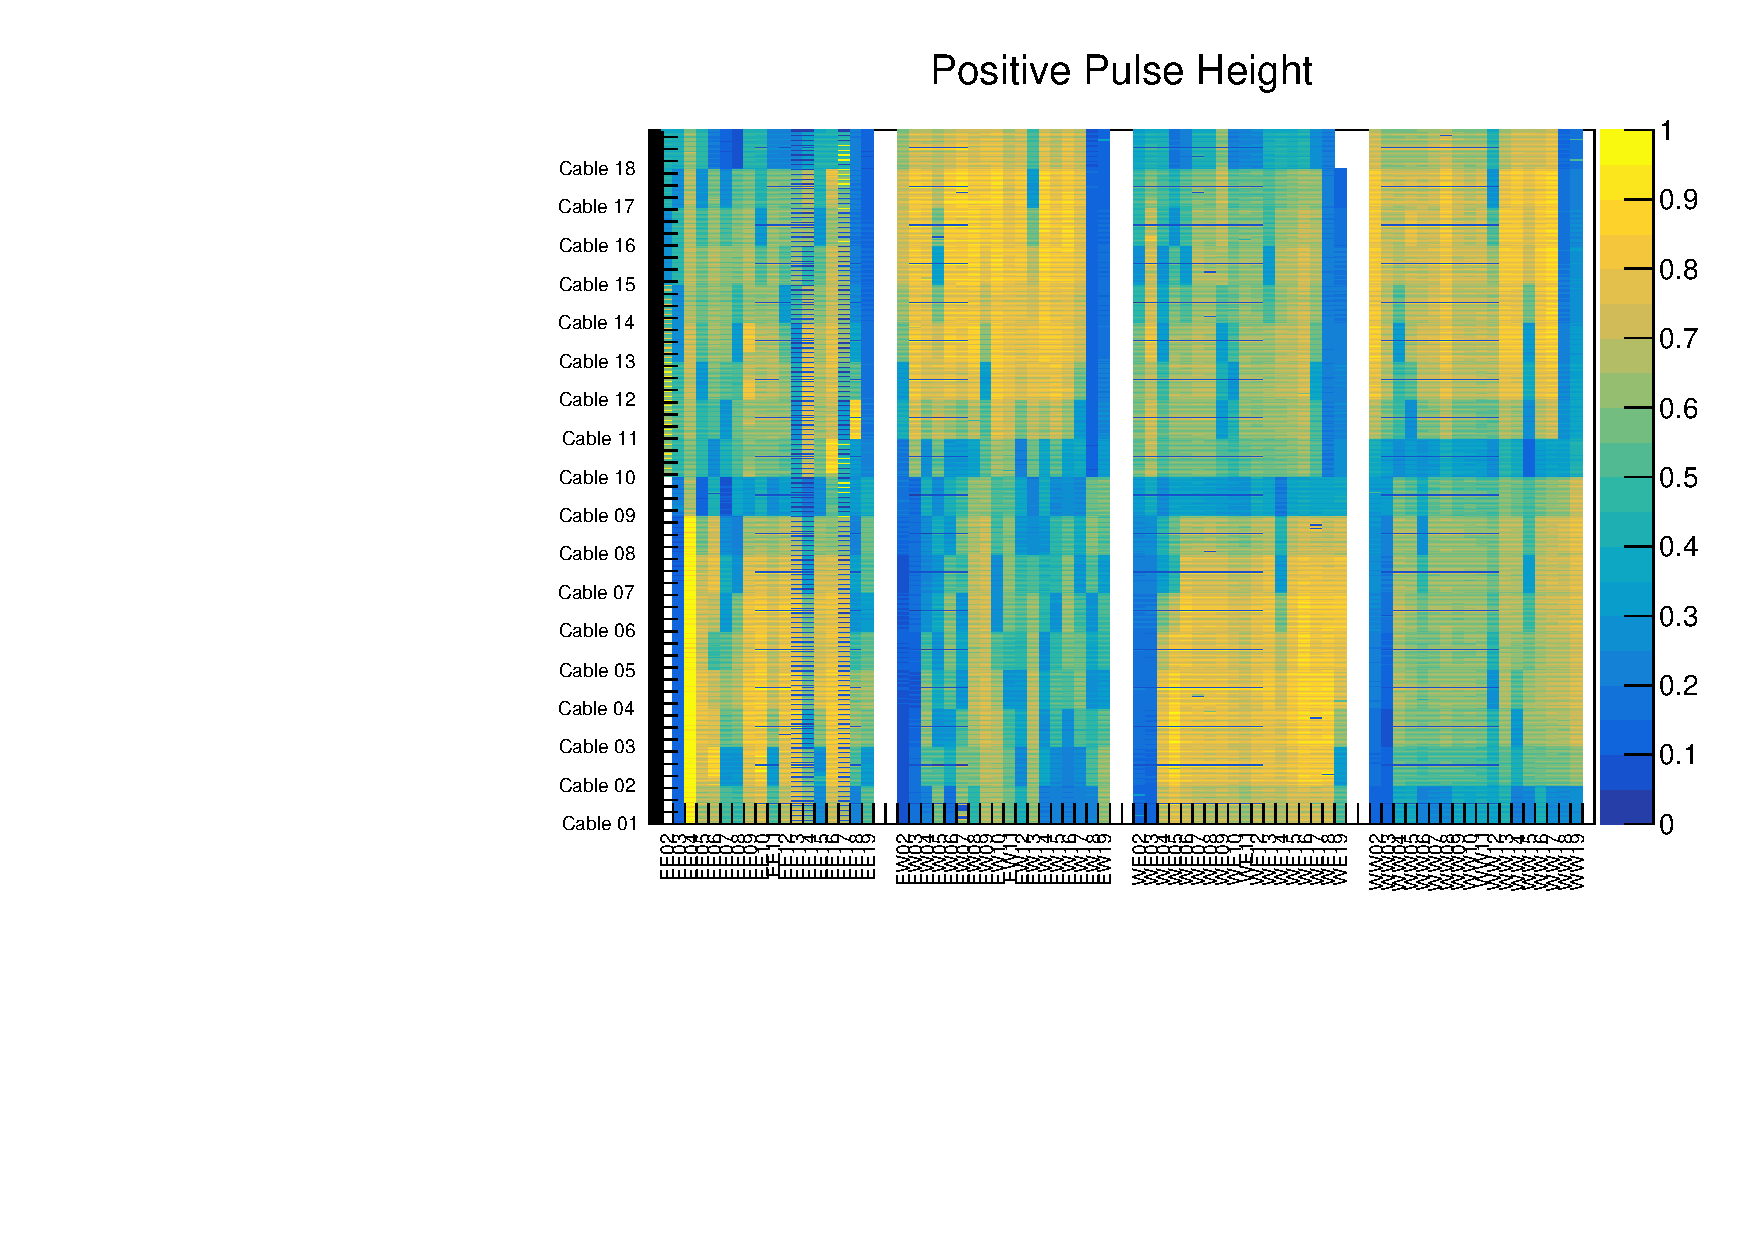
\includegraphics[width=\textwidth]{fig/PosPeak.pdf}
\caption{The map of the positive peak values of all the channels.
Each strip represents a single channel of the detector.
The x-axis includes all the chimneys of the ICARUS detector, while
the y-axis shows all the 18 cables, each with 32 channels, within a chimney.
The color code in each figure indicates the values of the positive peak.}
\label{fig:pospeak}
\end{figure}
% ----------------------------------------------------------------------

% ----------------------------------------------------------------------
\begin{figure}
\centering
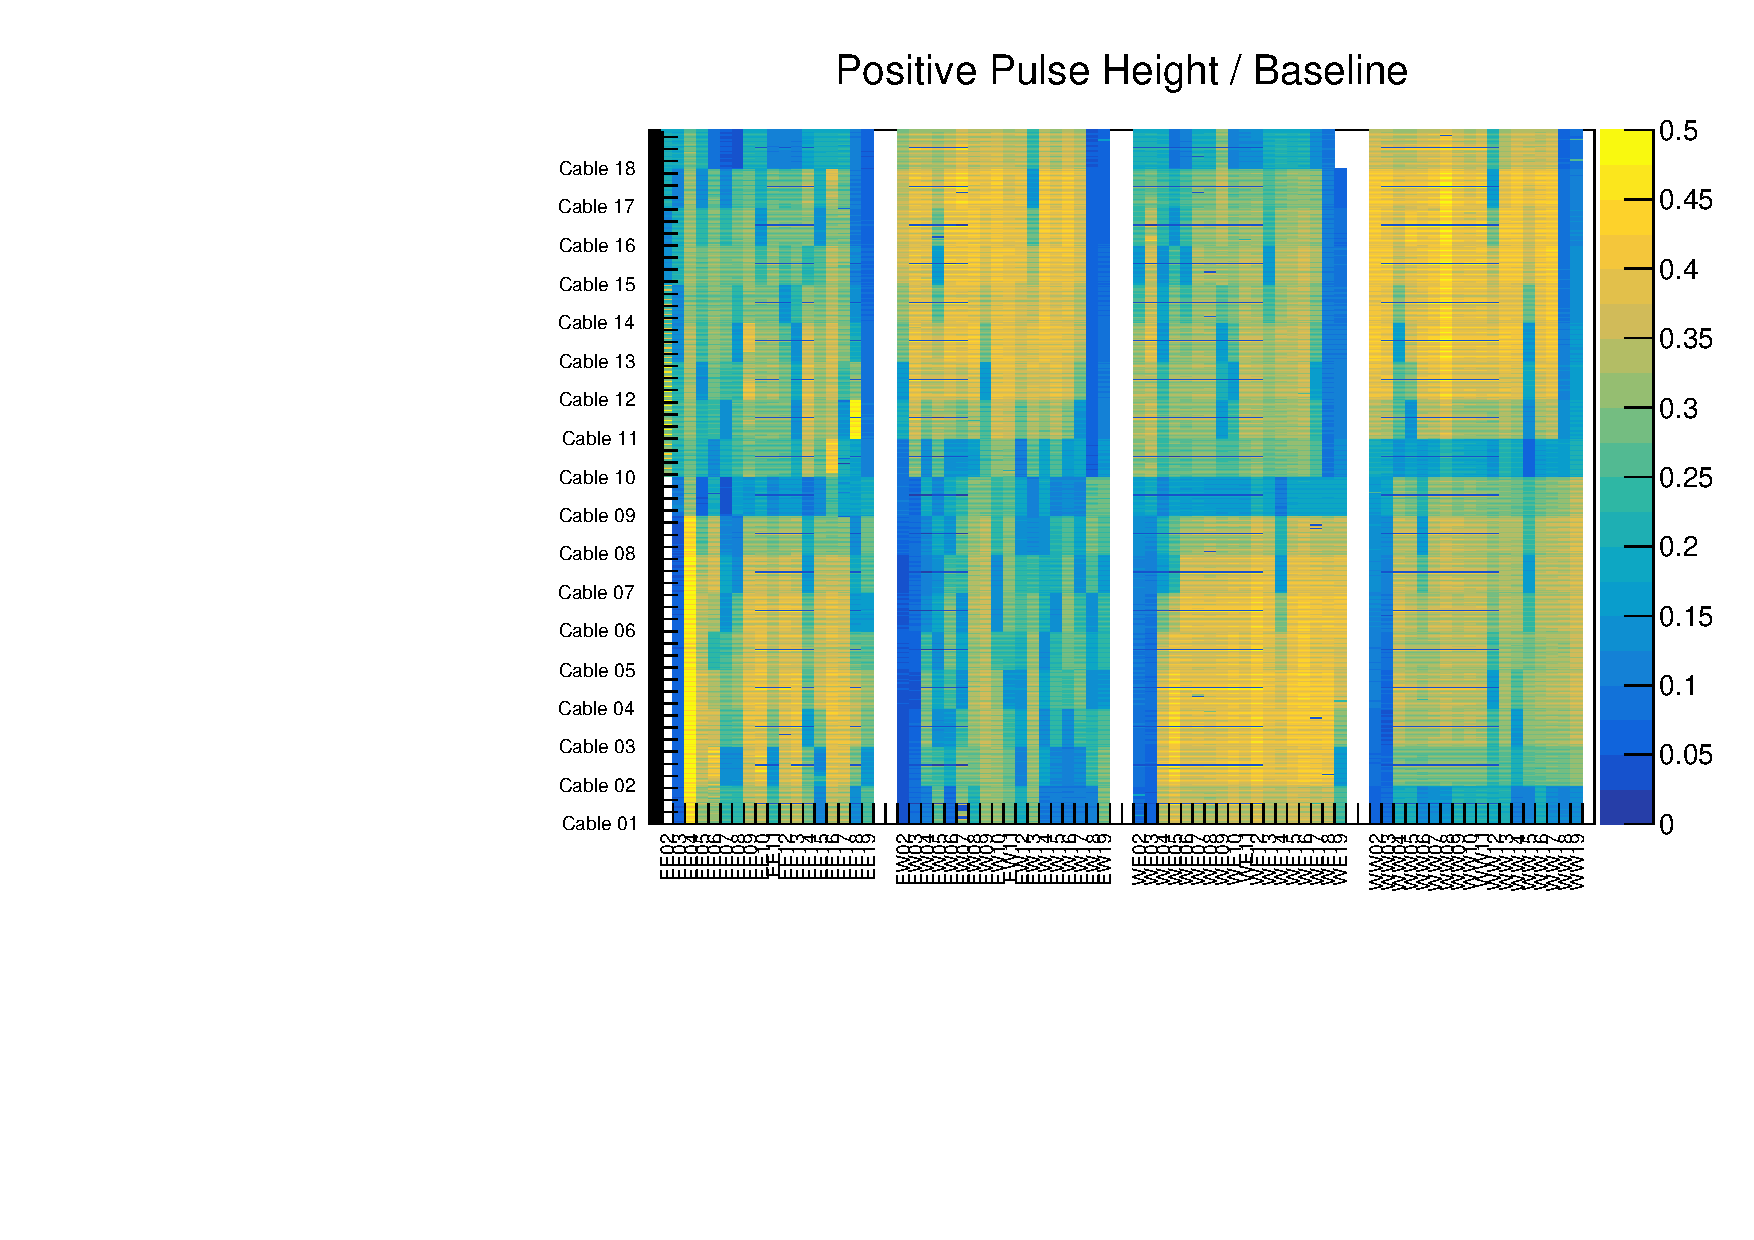
\includegraphics[width=\textwidth]{fig/PosPeakToBaseline.pdf}
\caption{The map of the positive peak to baseline ratios of all the channels.
Each strip represents a single channel of the detector.
The x-axis includes all the chimneys of the ICARUS detector, while
the y-axis shows all the 18 cables, each with 32 channels, within a chimney.
The color code in each figure indicates the values of the ratio.}
\label{fig:pospeaktobaseline}
\end{figure}
% ----------------------------------------------------------------------

% fine structure in the same cable
\Cref{fig:pospeaktobaseline} shows slight non-uniformity
in the signal amplitude of some cables, 
such as cables 10-13 in chimney EE09.
Looking into the values of those cables, we clarify those cables do not
have particularly non-uniform signal amplitudes, and the effect shown
in \Cref{fig:pospeaktobaseline} is rather owing to the color scale.\\

% conclusion
We conclude that there is no disconnected cable, and the source of all 
the cables with lower signal amplitude is confirmed to be the grounding.




\section{Interpretation of the results}
\label{sec:Results}

Histograms, shielded/non-shielded cable problems, cross-talk, etc....



\appendix

\section{Setup of acquisition code}
\label{app:DAQsoftwareSetup}

The data acquisition pattern followed in this test has been described in
\cref{ssec:streamlined-interactive-data-acquisition}.
In this section, technical details are described for the set up of the software
for that acquisition.

All the original code written by Sergi Castells and the following extensions are
published in a public GIT repository. A copy of that repository is currently
available in GitHub as
\href{https://github.com/PetrilloAtWork/ICARUSconnectivityTest}{\texttt{PetrilloAtWork/ICARUSconnectivityTest}}\footnote{%
URL: \url{https://github.com/PetrilloAtWork/ICARUSconnectivityTest}.}.
The software used for data acquisition in September 2018 was being developed as
the need arose. At the beginning, Sergi's code, roughly equivalent to the tag
\texttt{v01\_00} of the repository above, was used
directly. By the end of the data acquisition, version \texttt{v03\_00} was used,
and code was drawn from that version for the analysis as well.
In the following connectivity test, planned for December 2018, the starting
version will be \texttt{v04\_00} (see \cref{apx:DAQsoftwareSetup:Future}).

The test driver is unfortunately hard to correctly set up the first time.
The software is all written in python 2, and it requires both the python
Visual Instrument Software Architecture (PyVISA, exposing the module
\texttt{visa}) and CERN ROOT (PyROOT, exposing the module \texttt{ROOT})
interfaces. It proved hard to get to a configuration where python would
load both at the same time on OSX, while no Linux laptop was tried. The
pattern that seemed more likely to succeed was to install PyVISA
following online instructions found at
\url{https://pyvisa.readthedocs.io/en/master/index.html}, which
included installing National Instrument backend software\footnote{%
Registration to National Instruments web site is required in
order to download the software, but no fee payment was required to
download the driver package.
}, that we used in its release 18.0. After having tested that the \texttt{visa}
module correctly work, again as described in the linked documentation,
we compiled ROOT (6.14) from source \emph{in the same environment} (that
is, in the same shell).

The setup of the test instrumentation is the same as for the software
from Sergi. The data acquisition session is run within a single
\texttt{python} session. Its setup includes importing the test driver
module (\texttt{testDriver.py}), setting the IP address of the
oscilloscope in use, and finally instantiate the test driver. A possible
setup sequence is:
\begin{verbatim}
from testDriver import *
loadScopeReader('192.168.230.29')
reader = ChimneyReader()
\end{verbatim}
After this per-session setup, the data acquisition is driven by choosing
the chimney (e.g. \texttt{reader.start("EW09")}) and repeatedly call the
acquisition function (\texttt{reader.next()}). It is also possible to
skip to remove the last acquisition and repeat it, or skip to a
different one.

Note that for up-to-date instructions the file \texttt{README.md} in the GIT
repository supersedes the information provided here.


\subsection{Improvement implemented for December 2018 test}
\label{apx:DAQsoftwareSetup:Future}

This section shortly lists improvements that are implemented and will be tested
for the following connectivity test, the last without the official ICARUS DAQ,
planned for December 2018.
\begin{itemize}
  \item single script working for all oscilloscopes
  \item configuration of the script driven by configuration file(s)
  \item integrated verification of the correctness of the data format at the end
        of the acquisition from a chimney
  \item generation of a data transfer script
  \item single connection to the oscilloscope for the whole session (more error
        prone but \emph{much} faster; \texttt{ChimneyReader.scope().reconnect()}
        may help to recover connection issues
  \item ability to jump to a chosen cable and position at any time
        (\texttt{ChimneyReader.jumpTo()})
\end{itemize}
The expected acquisition flow is outlined as follows:
\begin{enumerate}
  \item preparation of the data acquisition: start of the python interactive
        shell, initialisation of `testDriver` helper object with the proper
        configuration file, selection of the first chimney to read out;
  \item sequential acquisition of waveforms from all cables, with the same
        pattern as in September 2018;
  \item after completion, verification of the data written on the local disk;
        this may take 5-10 minutes, while the operators may ``close'' the tested
        chimney and prepare for the acquisition of the next one (but note that
        if data is found incomplete, more acquisition might need to take place);
  \item after data is validated, generation of a data transfer script
  \item execution of the generated script into a separate shell, going in
        parallel with the rest of the activity
\end{enumerate}
The remote destination of the data is specified in the configuration file.


\section{Supporting library software}
\label{app:supporting-library-software}

The analysis is supported by a utility library which is available as GIT
repository, with the main repository being stored by GitHub at
\texttt{github.com:PetrilloAtWork/ICARUSconnectivityTest.git}. It is
possible to download it with:

\begin{verbatim}
git clone git@github.com:PetrilloAtWork/ICARUSconnectivityTest.git
\end{verbatim}

or equivalent.\\

The analysis library used for the online analysis is tagged as
\texttt{v03\_00}. In that version, both waveform parsing and analysis
code are in \texttt{drawWaveforms.py}.\\

Utility classes are provided:

\begin{itemize}
\tightlist
\item
  \texttt{WaveformSourceInfo}: a data structure describing a waveform by
  its parameters: chimney, connection, test box switch position,
  oscilloscope channel and index

  \begin{itemize}
  \tightlist
  \item
    \texttt{channel} attribute is provided with the number of connection
    channel, computed from the switch position and oscilloscope channel
    and ranging between \texttt{1} and \texttt{32}
  \item
    \texttt{increaseIndex()} is a shortcut to increase the index
    attribute
  \item
    \texttt{firstIndexOf(position)} is a static method returning the
    index of the first waveform on a given switch position
  \end{itemize}
\item
  \texttt{WaveformSourceParser}: a class that represents the group of
  waveform files which contains a specified one, the ``triggering
  file'':

  \begin{itemize}
  \tightlist
  \item
    the triggering file is specified at construction or with
    \texttt{parse()} method
  \item
    the parameters of the triggering files are accessible via
    \texttt{sourceInfo} (a \texttt{WaveformSourceInfo} instance)
  \item
    the pattern of the file path is stored as
    \texttt{sourceFilePattern}, and a full file name can be obtained by
    \texttt{sourceFilePattern\ \%\ sourceInfo} (with \texttt{sourceInfo}
    \emph{any} valid \texttt{WaveformSourceInfo})
  \item
    the list of expected names for all \texttt{N} files at the current
    (or the specified) oscilloscope channel can be obtained via
    \texttt{allChannelSources()}
  \item
    the list of expected names for all \texttt{4N} files at the current
    test box switch position can be obtained via
    \texttt{allPositionSources()}
  \end{itemize}
\end{itemize}

Plotting functions:

\begin{itemize}
\tightlist
\item
  \texttt{plotWaveformFromFile()} creates and returns a single
  \texttt{TGraph} with the specified waveforms
\item
  \texttt{plotAllPositionWaveforms()} returns a \texttt{TCanvas} split
  in as many pads as there are oscilloscope channels (\texttt{4}), and
  plots in each pad all the waveforms from a channel

  \begin{itemize}
  \tightlist
  \item
    the first argument is a \texttt{WaveformSourceParser} object which
    determines which waveforms are plotted (equivalent to
    \texttt{allPositionSources()})
  \item
    the vertical range of all graphs is fixed to be at least between 1
    and 3 volt
  \item
    statistics are extracted and printed in each pad, as documented
    below
  \end{itemize}
\item
  \texttt{plotAllPositionsAroundFile()} plots all the waveforms for the
  same connector and test box switch position as the one of the
  specified waveform file; the plots are described with
  \texttt{plotAllPositionWaveforms()} above
\end{itemize}

The statistics box of the plots includes: * ``waveforms'': the number
\texttt{N} of waveforms in the plot (typically 10) * ``baseline'': the
average of the \texttt{N} baselines of the \texttt{N} waveforms, each
one computed with \texttt{extractBaseline()} algorithm * ``RMS'': the
average of the \texttt{N} RMS on the baseline of the \texttt{N}
waveforms; this is a quantification of the average noise * ``maximum'':
for each waveform, the largest value is found; the \emph{maximum} is the
average of the distribution of maxima from the \texttt{N} waveforms, and
the uncertainty is its error * ``peak'': for each waveform, the positive
and negative peaks are found over the baseline, and the largest is used;
the \emph{peak} is the average of the distribution of single waveform
peaks * ``RMS'' is the RMS of that peak value distribution. \\

Additionally, a small statistics library is provided: *
\texttt{MinAccumulator}, \texttt{MaxAccumulator},
\texttt{ExtremeAccumutator}, \texttt{MinAccumulatorN},
\texttt{MaxAccumulatorN} and \texttt{ExtremeAccumutatorN} remember the
\emph{N} largest or smallest (or both) of the values that are
\texttt{add()}'ed to them * \texttt{StatAccumulator} gives average,
error, RMS and related quantites, of the sample given to it element by
element (via \texttt{add()} call) \\

The fundamental analysis algorithms applied on a single waveform are: *
\texttt{findMaximum()}, \texttt{findMinimum()} and
\texttt{findExtremes()} return the position respectively of the maximum,
of the minimum and of both, within the list of values in argument *
\texttt{extractBaselineFromPedestal()} extracts the baseline and its RMS
and uncertainty, as average of the samples in the start of the waveform
* \texttt{extractBaseline()} extracts the baseline of the waveform and
its RMS and uncertainty, as described in the previous section *
\texttt{extractPeaks()} extracts the value and location of the two peaks
of the waveform, with uncertainties, as described in the previous
section * \texttt{extractStatistics()} runs many of the previous
algorithms, and also select the absolute peak.


% uncomment when we actually have some references to refer to
% \bibliographystyle{plain}
% \bibliography{references} % check references.bib


\end{document}
%%%%%%%%%%%%%%%%%%%%%%%%%%%%%%%%%%%%%%%%%%%%%%%%%%%%%%%%%%%%%%%%%%%%%%%%%%%%%%%%
